\documentclass[10pt,letterpaper]{article}

\usepackage{ccn}
\usepackage{pslatex}
\usepackage{apacite}
\usepackage{graphicx}
\usepackage{caption}
\usepackage{natbib}
\usepackage{float}

\usepackage{hyperref}       % hyperlinks
\usepackage{url}            % simple URL typesetting
\usepackage{booktabs}       % professional-quality tables
\usepackage{amsfonts}       % blackboard math symbols
\usepackage{nicefrac}       % compact symbols for 1/2, etc.
\usepackage{microtype}      % microtypography
\usepackage{xcolor}         % colors
\usepackage{amsmath}
\usepackage{amssymb}
\usepackage{mathtools}
\usepackage{amsthm}
\usepackage{graphicx}
\usepackage[labelfont=bf, margin=0.8cm, font=sf]{caption}

\title{Collapse Around the Circuit: An Induction Head Survives Recursive Training While In-Context Generation Degrades}

\author{{\large \bf Author 1 } \\ University of the Witwatersrand, 1 Jan Smuts Ave,\\ Braamfontein, Johannesburg, 2000, South Africa
  \AND {\large \bf Author 2 } \\ University of the Witwatersrand, 1 Jan Smuts Ave,\\ Braamfontein, Johannesburg, 2000, South Africa
  \AND {\large \bf Author 3} \\ University of the Witwatersrand, 1 Jan Smuts Ave,\\ Braamfontein, Johannesburg, 2000, South Africa}


\begin{document}

\maketitle
\phantom{.}
\newpage
\phantom{.}
\newpage

\section{Abstract}
{
\bf
\looseness=-1
Induction heads are the mechanism widely credited with in-context learning (ICL) in transformers, and recursive training on model-generated data is known to cause model collapse, but whether collapse degrades the ICL circuit itself or only its downstream outputs is untested. We build the induction-head task of \citet{singh2024needs} and place a two-layer attention-only transformer in a multi-generation collapse pipeline, training a fresh model each generation on a pool mixed from real and self-generated data at a controlled real-data fraction. We track the circuit causally, by zero-ablating the heads responsible, alongside behavioural accuracy and generation diversity, across a task variant with one free generative choice. Over 6 generations, 5 real-data fractions and 3 seeds, the induction circuit stays fully intact and load-bearing at every fraction, while the model's free generative choice degrades in a graded, dose-dependent way, chiefly through growing probability mass on symbols never shown in context. The standard marginal-diversity metric is blind to this; a conditional, per-context diversity metric is not. We further show that attention-pattern probes alone falsely read some fresh models as ``collapsed'' circuits, because a subset of models solve the task with one of two non-canonical algorithms that a causal probe correctly credits. Collapse, in this setting, happens around the induction circuit rather than inside it.
}
\begin{quote}
\small
\textbf{Keywords:}
in-context learning; induction heads; model collapse
\end{quote}

\section{Introduction} \label{Intro}
\looseness=-1
Large language models can adapt to a pattern shown only in their prompt, without any weight update. \citet{olsson2022context} attribute much of this in-context learning (ICL) to \emph{induction heads}: a previous-token head that copies the token preceding each position, feeding an induction head one layer later that finds an earlier occurrence of the current token and copies whatever followed it. \citet{singh2024needs} isolate this circuit in a minimal symbol-copying task and characterise the architectural and training conditions under which it forms. Separately, \citet{shumailov2023curse,shumailov2024ai} show that models trained recursively on their own (or their predecessors') generations suffer \emph{model collapse}: successive generations lose the tails of the true data distribution and contract towards their own most probable outputs. Both literatures study transformers under training dynamics, but they have not been combined: does recursive self-training degrade the induction circuit itself, or does it degrade only what a still-intact circuit is asked to produce? We answer this using \citeauthor{singh2024needs}'s own task, extended so that part of every generation's output is a free choice rather than a fixed copy target, and track the circuit causally rather than only behaviourally.

\subsubsection{Background}
\looseness=-1
The induction circuit is a two-step composition: a previous-token head (layer 0) writes the preceding token's identity into each position; an induction head (layer 1) then attends, from the current token, to the earlier position carrying a matching identity, and copies what follows it \citep{olsson2022context,singh2024needs}. Attention patterns are the usual evidence for such a circuit, but \citet{conmy2023towards} note that pattern-reading is not causal evidence; we adopt their remedy, zero-ablation, throughout. Model collapse is normally diagnosed behaviourally, e.g. by falling output diversity or perplexity on held-out real data \citep{shumailov2024ai}; we instead ask the diagnosis of the mechanism directly.

\section{Methods}
\looseness=-1
\textbf{Task.} We use \citeauthor{singh2024needs}'s study$\to$query symbol task: $K{=}4$ symbols (drawn from a pool of 16) are each given a random label (from 6) for one sequence only; a study block presents the $K$ pairs in one order, a query block re-presents the same symbols in an \emph{independent} order with labels withheld. Because the match offset varies with the query permutation, only content-based matching -- not a fixed positional shortcut -- solves the task. In \emph{extended} mode the model additionally free-generates one more symbol from the $K$ shown, and its label, which we call $sq2$; $sq2$ is drawn uniformly at random and is therefore irreducible to predict, giving a provable loss floor of $\ln K/(K{+}2) \approx 0.231$ for $K{=}4$ (confirmed for $K \in \{2,\ldots,5\}$, independent of vocabulary size). This clean circuit also required rotary position embeddings (previous-token attention plateaus at $\sim$0.3 with absolute positions), tied input/output embeddings, and a cosine-decayed learning rate (a constant rate destabilises an already-formed circuit).

\textbf{Model.} A 2-layer, 4-head, attention-only transformer ($d{=}64$, $\sim$35.6k parameters). Hyper-parameters (lr, warmup, width) were grid-searched against validation loss (2 seeds), then confirmed on a disjoint seed. In extended mode most configurations sit at the loss floor, making validation loss near-uninformative: the top-ranked configuration in fact failed to form the circuit on the held-out seed (test accuracy 0.63), motivating the convergence gate below.

\textbf{Collapse pipeline.} Generation 0 trains on fresh real data. Generation $g{\geq}1$ trains a \emph{fresh} model on a 20k-sequence pool of a controlled \texttt{real\_fraction} of fresh real sequences plus the remainder sampled from generation $g{-}1$ (every answer slot model-generated); 10\% of each pool is held out for validation, and test is fresh real data. Because extended-mode transition timing is seed-dependent (900--2900 steps; one seed never transitioned within 6000), each generation must clear a validation-accuracy gate or retrain from a new initialisation (up to 3 retries), so an undertrained generation is never misread as collapse. We sweep \texttt{real\_fraction} $\in \{0, 0.1, 0.25, 0.5, 1\}$ for 6 generations and 3 seeds, base and extended.

\textbf{Metrics.} Behavioural: query accuracy, generated-label accuracy. Distributional: \emph{marginal} diversity (entropy of $sq2$ over all symbols) is blind to collapse here because $sq2$ is always one of the $K$ in-context symbols, themselves a uniform draw, so its marginal stays near-uniform even if the model deterministically copies (say) the first study pair; we instead report \emph{conditional} diversity (entropy of $p(sq2\mid\text{context})$ over the $K$ in-context symbols, normalised by $\ln K$) and \emph{off-context mass} (probability placed on symbols never shown). Mechanistic: for every saved model we compute each head's attention to the matching label position and to several fixed-offset controls, then zero-ablate individual heads and whole layers to obtain a causal accuracy drop (Figure~\ref{fig:circuit}), which we show below is necessary because attention patterns alone can mis-classify the algorithm a model actually uses.

\begin{figure}[h!]
  \captionsetup{margin=0.0in, font=sf}
  \begin{minipage}{\linewidth}
  \centering
    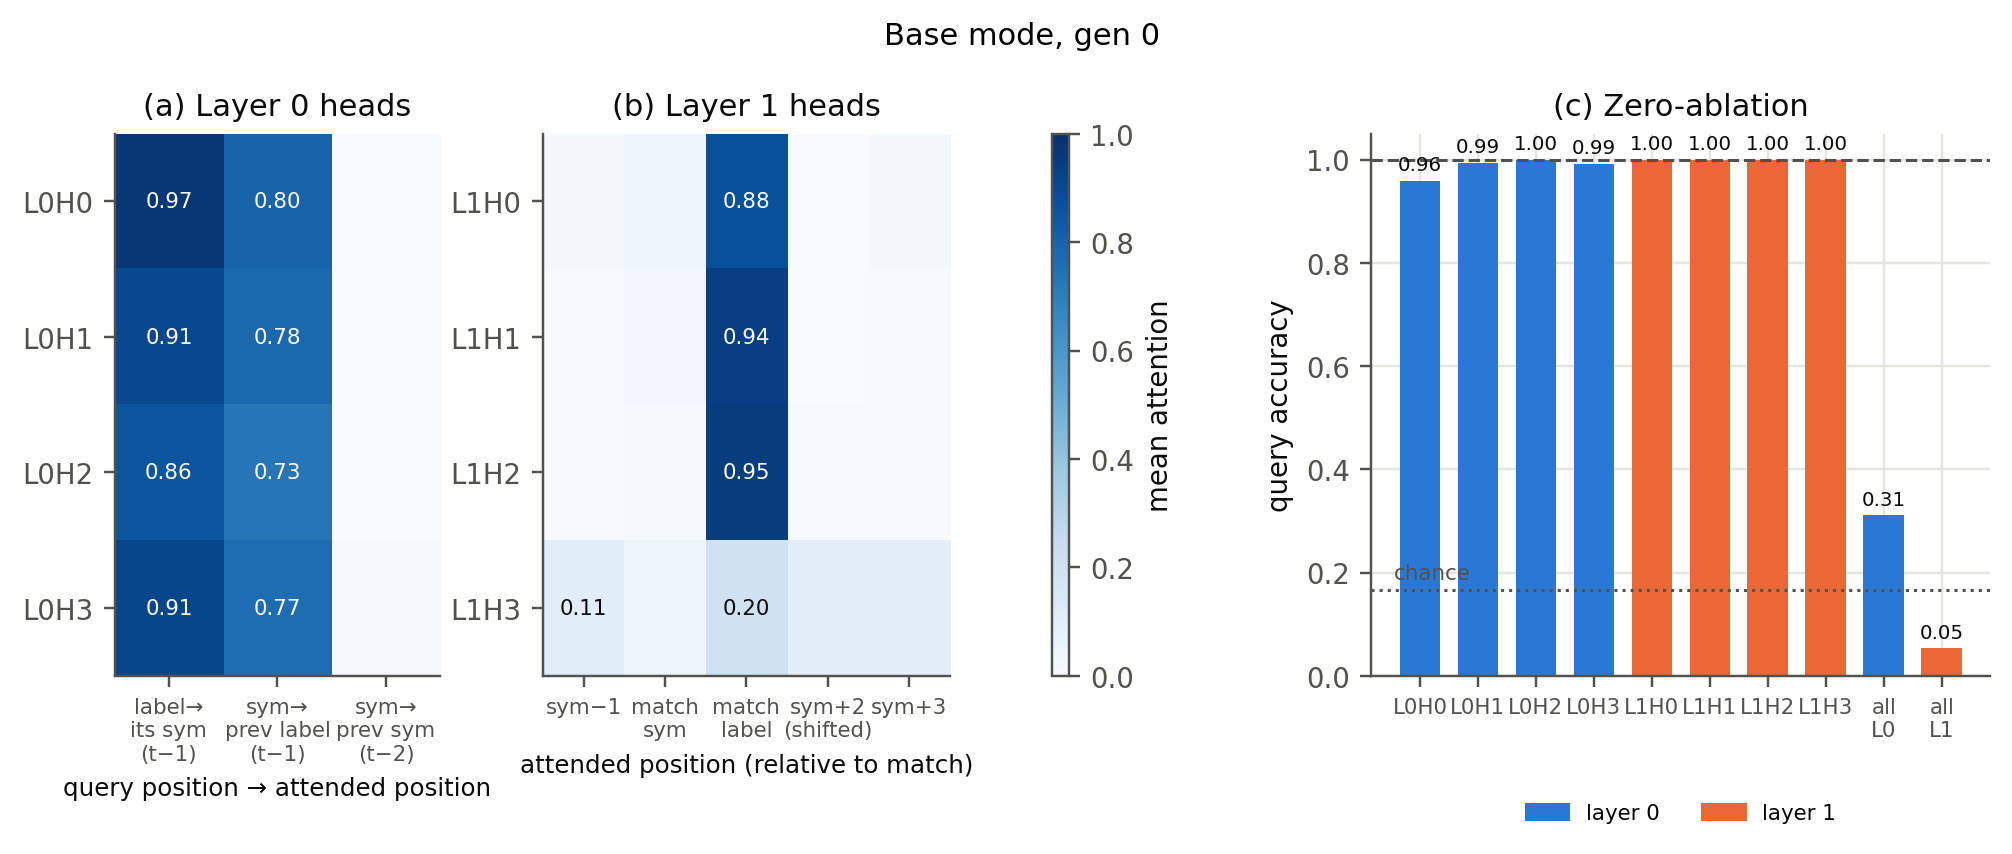
\includegraphics[width=1.0\linewidth]{figures/fig_circuit_base.png}
  \end{minipage}
  \caption{\looseness=-1 Base-mode circuit, generation 0. (a) All four layer-0 heads act as previous-token heads (attention 0.86--0.97). (b) Three of four layer-1 heads attend, from the query, to the matching label (0.88--0.95), not the matching symbol or a fixed offset -- ruling out a positional/direct-match shortcut. (c) Single-head ablation leaves accuracy $\geq$0.96; ablating all of layer 0 drops it to 0.31, all of layer 1 to 0.05 -- causally load-bearing and redundant within each layer.}
  \label{fig:circuit}
\end{figure}

\section{Results}
\looseness=-1
Table~\ref{tab:results} reports extended-mode conditional diversity, off-context mass, induction strength and query accuracy at the final generation, mean $\pm$ sd over 3 seeds (generation 0, fresh data: conditional diversity 0.994, off-context mass 0.012). Marginal diversity stays at 1.000--1.009 at every fraction and generation -- entirely uninformative here. The base-mode control (which has no free generative slot) stays at query accuracy $\geq$0.997 with induction strength 0.84--0.96 and no trend with \texttt{real\_fraction}.

\begin{center}
\small
\captionsetup{type=table, font=sf, width=0.95\linewidth}
\captionof{table}{\looseness=-1 Extended mode, final generation (mean $\pm$ sd, 3 seeds). Conditional diversity and off-context mass move together and monotonically with \texttt{real\_fraction}; induction strength and query accuracy do not.}
\label{tab:results}
\resizebox{\linewidth}{!}{%
\begin{tabular}{|c|c|c|c|c|}
\hline
real frac. & cond. div. & off-ctx mass & induction & query acc \\
\hline\hline
0.0  & 0.819 $\pm$ 0.022 & 0.052 $\pm$ 0.005 & 0.959 & 1.000 \\
\hline
0.1  & 0.858 $\pm$ 0.018 & 0.044 $\pm$ 0.003 & 0.965 & 1.000 \\
\hline
0.25 & 0.861 $\pm$ 0.026 & 0.031 $\pm$ 0.003 & 0.969 & 1.000 \\
\hline
0.5  & 0.898 $\pm$ 0.032 & 0.022 $\pm$ 0.003 & 0.955 & 1.000 \\
\hline
1.0  & 0.897 $\pm$ 0.018 & 0.012 $\pm$ 0.001 & 0.938 & 1.000 \\
\hline
\end{tabular}%
}
\end{center}

Figure~\ref{fig:dose} shows this as a dose-response: conditional diversity and off-context mass move smoothly with \texttt{real\_fraction} (no sharp critical fraction), while induction strength for both modes sits in a narrow, flat band throughout. Re-probing all 30 saved final-generation models confirms this causally: every one retains a canonical or near-canonical circuit, with whole-layer-1 ablation costing 0.74--1.00 accuracy (extended) / 0.61--0.93 (base). Two checks matter for these numbers. A finite-data confound: even \texttt{real\_fraction}$=$1 drops conditional diversity from 0.994 (generation 0, unlimited data) to $\sim$0.90 once generation $\geq$1 trains on a finite 20k pool ($\sim$77 epochs) -- the recursive effect is the residual gap to this control, not the raw drop from generation 0. Circuit multiplicity: 10/90 extended and 6/90 base generations converge on a non-canonical but fully accurate algorithm -- a ``shifted'' copy (via a $t{-}2$ head) or an ``elimination'' strategy (attending \emph{away} from the match, suppressing non-matches) -- and attention-pattern reading alone falsely calls 9 and 6 of these collapsed, though ablation shows both are load-bearing.

\begin{figure}[h!]
  \captionsetup{margin=0.0in, font=sf}
  \begin{minipage}{\linewidth}
  \centering
    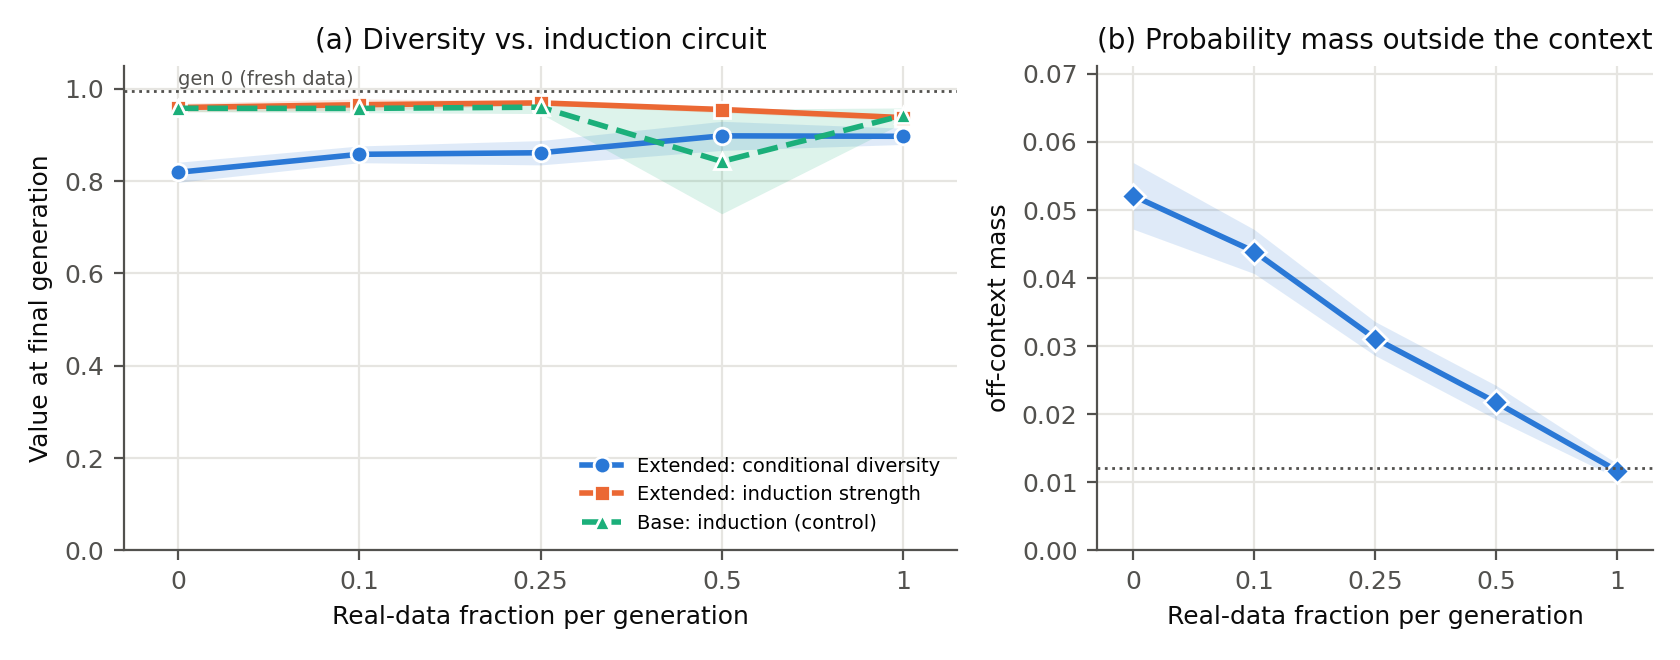
\includegraphics[width=1.0\linewidth]{figures/fig_dose_response.png}
  \end{minipage}
  \caption{\looseness=-1 (a) Extended-mode conditional diversity (blue) sits below the generation-0 ceiling and rises only gradually with \texttt{real\_fraction}, while induction strength (orange; green for the base control) stays flat near 0.94--0.97. (b) Off-context mass -- probability placed on symbols never shown -- falls smoothly from $\sim$0.05 at \texttt{real\_fraction}$=$0 to the generation-0 floor of 0.012 at $=$1: the clearest single symptom of collapse here.}
  \label{fig:dose}
\end{figure}

\section{Discussion}
\looseness=-1
Recursive training here produces a \emph{dissociation}, our answer to the question posed in the introduction: the ICL circuit is not what collapses. Query labels are fixed by the context, so every self-generated sequence re-validates the same copy computation; $sq2$ is under-determined, so a model's own sampling noise feeds its successor's training signal, and collapse concentrates there -- chiefly as \emph{off-context hallucination} (mass on symbols never shown) rather than a sharper-but-still-in-context preference. The dose-response is graded, not critical: $\sim$50\% real data already matches the all-real control on diversity, while off-context mass keeps improving up to \texttt{real\_fraction}$=$1, so no single fraction marks a break. Two points generalise beyond this task: marginal diversity is blind whenever the generative slot is a uniform draw over context-dependent options, so auditing an ICL model for collapse needs a \emph{conditional} diagnostic; and an attention-pattern probe is algorithm-specific, so causal ablation -- not pattern-reading -- should license any claim that a circuit has degraded. Limitations: a 35.6k-parameter model, 16-symbol vocabulary, 6 generations, 3 seeds, temperature 1 only, zero- (not mean-) ablation, and shared generation-1 seeds across fractions (so one unlucky initialisation, e.g. seed 2's elimination-circuit run, recurs at every fraction). What the $sq2$ sharpening is keyed on beyond context membership is unidentified (study-/query-slot entropies stay near 1); we leave this, and a seeded symbol-bias amplification probe, to future work.

\section{Acknowledgements (Not in Page Limit -- you will probably not have one)}
Computations were performed using High Performance Computing infrastructure provided by the Mathematical Sciences Support Unit at the University of the Witwatersrand.

\section{Contribution Statements (Not in Page Limit)}
TODO: fill in before submission -- all authors must agree on this text.

Do not forget to include the NeurIPS Checklist and the Wits Science Faculty AI Ethics Form.

\bibliographystyle{apacite}

\setlength{\bibleftmargin}{.125in}
\setlength{\bibindent}{-\bibleftmargin}

\bibliography{references}


\end{document}
